\documentclass[ngerman,a4paper,twocolumn,twoside]{scrartcl}
\usepackage[ngerman]{babel}
\usepackage{fontspec}
\usepackage[sfdefault,condensed]{roboto}
\usepackage{pifont}
\usepackage{csquotes}
\usepackage{hyperref}
\usepackage{amsmath}
\usepackage{url}
\usepackage{mhchem}
\usepackage{siunitx}
\sisetup{locale=DE}
\usepackage{graphicx}
\usepackage{cleveref}
\usepackage{scrlayer-scrpage}
\usepackage[left=2cm, right=2cm, top=2cm, bottom=2cm, foot=1cm]{geometry}

\graphicspath{{graphics/}}

\title{Ergänzungen zum Versuch 501 -- Röntgenspektren und Compton-Effekt}
\subtitle{Betreffend Versuchsteil 1.3 bzw. 3.4 (Wellenlängenverschiebung durch Compton-Effekt)}
\author{\url{https://git.io/fj3zp} -- Revision \texttt{3a0d269
}}
\begin{document}
\maketitle
\subsection*{Hintergrund}
Die folgenden Anmerkungen sollen der Klarstellung des Versuchsteils zum Compton-Effekt dienen. Sie basieren auf der Versuchsanleitung des Herstellers\footnote{Leybold-Didactic zu finden unter \url{http://www.ld-didactic.de/documents/de-DE/EXP/P/P6/P6371_d.pdf}} mit Ergänzungen betreffend der Korrektur der Wellenlängenverschiebung infolge der elastischen Streuung.
\subsection*{Versuchsidee}
Der Compton-Effekt beschreibt die inelastische Streuung von Photonen an Elektronen. Dabei geben die Photonen einen Teil ihres Impulses $p=h/\lambda$ (und damit auch ihrer Energie $E=hf$) an das Elektron ab. Interessanterweise hängt die Änderung der Wellenlänge $\Delta\lambda$ dabei nur vom Winkel $\vartheta$ ab, unter dem das Photon relativ zu seiner Einfallsrichtung gestreut wurde:
\begin{align}
\Delta\lambda=\lambda_2-\lambda_1=\lambda_C \cdot (1-\cos\vartheta), \label{eq:compton}
\end{align}
Compton-Wellenlänge $\lambda_C\approx\SI{2.426e-12}{\m}$
\par
Im Versuch wird quasi monochromatische Röntgenstrahlung verwendet. Aus den Vorversuchen ist bekannt, dass die Anode ein breites Spektrum mit Bremsstrahlungsuntergrund und mindestens zwei charakteristischen Linien erzeugt. Zur \emph{Monochromasierung} könnte z.B. ein Kristall verwendet werden (siehe Bragg Bedingung), wodurch sich allerdings die Intensität stark verringern würde. Stattdessen nutzt man eine typische Eigenschaft von Materialien: Die K-Absorptionskante des um ein oder zwei Ordnungszahlen kleineren Elements lässt quasi nur die $\mathrm{K}_\alpha$ Strahlung passieren (hier \ce{_{40}Zr} zur Filterung der charakteristischen Strahlung von  \ce{_{42}Mo} -- vergleiche die gemessenen Kurven). Für alle folgenden Überlegungen betrachten wir den Zirkonium-Filter als Teil der Quelle. Dabei ist zu beachten, dass die so erhaltene Strahlung trotzdem eine recht große Bandbreite aufweist (kann direkt aus der Messung der Strahlung mit Zr Filter entnommen werden). Insofern wird im Folgenden von \emph{mittleren Wellenlängen} gesprochen die sich nahe der ursprünglichen Wellenlänge der $\mathrm{K}_\alpha$ Linie von Molybdän befinden.
\par
Aus dem Vorversuch ist weiterhin bekannt, dass für die Transmission des Kupferabsorbers (mit bekannter Dicke $D$ und Kernladungszahl $Z$) gilt:
\begin{align}
I&=I_0e^{-\gamma{}D}=I_0e^{-(\mu+\sigma)D} \\
\Rightarrow T&=\frac{I}{I_0}\propto e^{-\mu} \propto e^{-\lambda^3}.
\end{align}
In Worten: Die Transmission des Kupferabsorbers reagiert empfindlich (exponentiell mit der dritten Potenz) auf kleine Änderungen der Wellenlänge. Weiterhin gibt es nahe der untersuchten Wellenlänge, bei der eine solche kleine Änderung (Compton-Streuung) gezeigt werden soll, keine Absorptionskante. Die K-Absorptionskante von Kupfer liegt erst bei etwa \SI{138}{\pico\meter}, insofern kann von einem bijektiv-stetigen Verlauf ohne Sprünge ausgegangen werden. Dann ist folgender Versuch denkbar:
\begin{enumerate}
\item Streue die monochromatische Röntgenstrahlung an einer Aluminium-Probe. Es kommt zu einer minimalen Verschiebung der Wellenlänge infolge des Compton Effektes.
\item Messe die Zählrate $R_0$ ohne Kupferabsorber um später die Transmission zu bestimmten.
\item Messe die Zählrate $R_1$,  wobei der Kupferdurchgang \textbf{vor} der Compton-Streuung stattfindet, d.h. Transmission der ungestreuten Wellenlänge.
\item Messe die Zählrate $R_2$, wobei der Kupferdurchgang \textbf{nach} der Compton-Streuung stattfindet, d.h. Transmission der gestreuten Wellenlänge.
\end{enumerate}
Dann kann mithilfe der Transmissionskurve der Kupfer-Probe $T(\lambda)$ bzw. ihrer Umkehrung $\lambda(T)$ bestimmt werden, wie stark die Wellenlänge sich bei der Compton Streuung ändert:
\begin{align}
\Delta\lambda&=\lambda_2 - \lambda_1=\lambda(T_2)-\lambda(T_1)\\&=\lambda\left(\frac{R_2}{R_0}\right)-\lambda\left(\frac{R_1}{R_0}\right)
\end{align}
Da manchmal eine Zeichnung mehr sagt als tausend Worte, ist das hier noch einmal grafisch dargestellt:
\begin{figure}[h!]
\centering
\input{graphics/Sketch.pdf_tex}\\
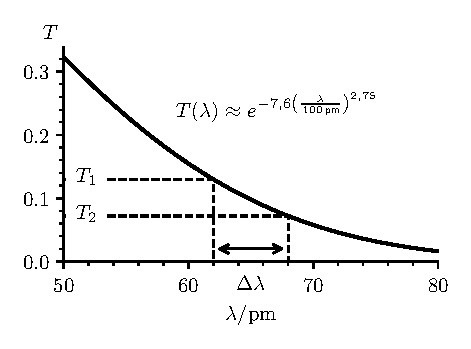
\includegraphics{plot.pdf}
\caption{Vereinfachte Darstellung des Experiments.}
\end{figure}
\subsection*{Durchführung}
Im Prinzip lässt sich der Versuch wie oben beschrieben durchführen. Es gibt allerdings noch ein paar \enquote{Klimmzüge} aufgrund der geringen Änderung der Wellenlänge zu schaffen:
\begin{itemize}
\item Die Zählzeiten müssen vergleichsweise lang sein.
\item Die Nullrate $R_N$ muss berücksichtigt werden.
\item Der Fehler infolge von elastischer Streuung muss mathematisch korrigiert werden.
\end{itemize}
Wie diskutiert, wird der Zirkoniumfilter für diesen Versuchsteil dauerhaft eingesetzt. Es bietet sich an, diesen auf der Rückseite des Kollimators einzusetzen -- dieser kann dazu entnommen werden. Dann wird die Aluminiumprobe eingesetzt und folgende Parameter eingestellt:
\begin{itemize}
\item Targetwinkel \SI{20}{\degree} (Taste \enquote{TARGET})
\item Sensorwinkel \SI{145}{\degree} (Taste \enquote{SENSOR})
\item Spannung $U=\SI{30}{\kilo\volt}$
\item Strom $I_e=\SI{1.00}{\milli\ampere}$ (außer Nullrate)
\item Schrittweite $\Delta\beta=\SI{0.0}{\degree}$
\item Meszeit $\Delta t=\SI{500}{\s}$
\end{itemize}
Es werden vier Messungen durchgeführt (Zirkoniumfilter ist immer dabei):
\begin{enumerate}
\item Anordnung ohne Kupferabsorber liefert $R_0'$
\item Anordnung mit Kupferabsorber auf der Strahleintrittsseite liefert $R_1'$
\item Anordnung mit Kupferabsorber auf der Sensorseite liefert $R_2'$
\item Anordnung ohne Kupferabsorber und mit Emissionsstrom $I_e=\SI{0.00}{\milli\ampere}$ liefert die Nullrate $R_N$
\end{enumerate}
Die gestrichenen Raten $R_x'$ deuten an, dass die entsprechenden Werte noch nicht bezüglich der Nullrate korrigiert sind.
\subsection*{Auswertung}
Zunächst können unter Berücksichtigung der Nullrate die Transmissionen berechnet werden. Es gilt $R_x=R_x'-R_N$, wobei angenommen wird, dass die Intensität der Strahlung proportional zu korrigierten Zählrate ist, also $I_x \propto R_x$:
\begin{align}
T_1= \frac{I_1}{I_0} = \frac{R_1'-R_N}{R_0'-R_N} \;\;\text{und}\;\; T_2= \frac{I_2}{I_0} = \frac{R_2'-R_N}{R_0'-R_N}.
\end{align}
Nun muss ein geeignetes Modell $T(\lambda)$ gefunden werden, um aus der gemessenen Transmissionskurve des Kupferfilters nahe der $\mathrm{K}_\alpha$ Linie die zugehörigen Wellenlängen bestimmen zu können. Es bietet sich eine Funktion der Form
\begin{align}
T(\lambda) = \exp\left[-a\cdot\left(\frac{\lambda}{\SI{100}{\pico\meter}}\right)^b\right]
\end{align}
mit einheitenlosen Parametern $a$ und $b$ an. Dieses kann an die gemessenen Werte für $T_\text{Cu}$  in einem geeigneten Bereich (z.B. zwischen \SI{40}{\pico\meter} und \SI{70}{\pico\meter}) angepasst werden\footnote{Als Startparameter für die Kurvenanpassung können $a=\num{7.6}$ und $b=\num{2.75}$ gewählt werden}. Dies liefert die beiden Parameter $a$ und $b$ inklusive ihrer Unsicherheiten.
\par
Aus der Umkehrung der Funktion ergibt sich:
\begin{align}
\lambda(T)=\SI{100}{\pico\meter}\cdot\left(-\frac{\ln(T)}{a}\right)^{1/b}.
\end{align}
Die gesuchte Änderung der Wellenlänge durch Compton-Streuung ergibt sich letztlich aus:
\begin{align}
\Delta \lambda&= \lambda(T_2) - \lambda(T_1) \\
&=\SI{100}{\pico\meter}\left[\left(-\frac{\ln(T_2)}{a}\right)^{1/b}-\left(-\frac{\ln(T_1)}{a}\right)^{1/b}\right]  \label{eq:allgemeindeltalabda}\\
&=\frac{\SI{100}{\pico\meter}}{a^{1/b}}\left[(\ln(R_0'-R_N)-\ln(R_2'-R_N))^{1/b}\right.\notag\\&\phantom{=\frac{\SI{100}{\pico\meter}}{a^{1/b}}}\left.-(\ln(R_0'-R_N)-\ln(R_1'-R_N))^{1/b}\right]
\end{align}
und kann mit dem Ergebnis aus \cref{eq:compton} verglichen werden. Die Fehlerfortpflanzung ist nicht trivial zu berechnen -- es empfiehlt sich die Größen $a$ und $b$ als exakt anzunehmen und eventuell mit Zwischenergebnissen zu arbeiten.
\par
Zuletzt wird die in Aufgabenteil 3.4.3 angedeutete Korrektur durchgeführt, die berücksichtigt, dass der gemessene Wert von $R_2$ auch einen gewissen Anteil aus elastischer Streuung enthält (es sollte der rein inelastisch gestreute Anteil gemessen werden). Das Modell hierfür ist simpel:
\begin{align}
I_2 &\approx C \cdot I_1 + (1-C) I_2^\text{korr} \qquad &\text{d.h.}\\
R_2 &\approx C \cdot R_1 + (1-C) R_2^\text{korr} &| \div R_0 \\
T_2 &\approx C \cdot T_1 + (1-C) T_2^\text{korr} \label{eq:korrekturzwischenschritt}
\end{align}
Der Parameter $C\in [0,1]$ gibt an, mit welchem Anteil der elastisch gestreute Anteil ($R_1\propto I_1$) beiträgt. Der zweite Summand enthält den rein inelastisch gestreuten Anteil $R_2^\text{korr}$, welcher gesucht ist. Für $C=0$ wäre die inelastische Streuung perfekt, für $C=1$ tritt sie gänzlich nicht auf. Für den verwendeten Streuwinkel von $\SI{145}{\degree}$ gilt etwa $\frac{1-C}{C}\approx\num{2.23}$, d.h. $C\approx\num{0.3096}$. \Cref{eq:korrekturzwischenschritt} kann umgestellt werden zu
\begin{align}
T_2^\text{korr} = \frac{T_2-C\cdot T_1}{1-C}. \label{eq:korrektur}
\end{align}
Mit den erhaltenen Werten für $T_2^\text{korr}$ und der zugehörigen Unsicherheit kann erneut \cref{eq:allgemeindeltalabda} benutzt werden um $\Delta \lambda^\text{korr}$ zu erhalten.
\subsection*{Hinweis zur Fehlerrechnung}
Es sei noch einmal erwähnt, dass eine ordnungsgemäße Fehlerrechnung in diesem Fall durchaus kompliziert wäre, da beachtet werden muss, dass Zwischenergebnisse nicht ohne weiteres mit ihren \enquote{Zwischenunsicherheiten} verrechnet werden können. Dies ist nur möglich wenn die verrechneten Größen in den Rechnungen unterschiedlich sind -- anderenfalls könnten sich Fehleranteile möglicherweise in einem späteren Rechenschritt aufheben. Als Beispiel sei hier angeführt $x=4y-2y$, was sich formal zerlegen ließe als $x=u-v$, wobei $u=4y, \Delta u=4\Delta y$ und $v=2y, \Delta v=2\Delta y$. Dann erhält man insgesamt $\Delta x = \Delta u + \Delta v=6\Delta y$, was falsch ist, da man schon aus der Ausgangsformel sieht, dass $\Delta x=2\Delta y$. Der Fehler entsteht bei einer Zerlegung in Zwischenergebnisse, die eine nicht-disjunkte Menge von Messgrößen verrechnen. Im vorliegenden Fall führte kein Weg daran vorbei, \cref{eq:korrektur} in \cref{eq:allgemeindeltalabda} einzusetzen und nach allen fehlerbehafteten Größen ($R_0',R_1',R_2',R_N,a,b$) partiell abzuleiten...
\par
Im Rahmen des Grundpraktikums ist es zweckmäßig darüber hinwegzusehen. Allerdings kann es dadurch zu einer übermäßigen Akkumulation von Fehleranteilen kommen -- dies ist in der Diskussion zu beachten.
\par
Heutzutage wird stattdessen meist auf computergestützte Methoden zurückgegriffen. So gibt es für viele namhaften Programmiersprachen mit breiter wissenschaftlicher Nutzerbasis auch entsprechende Bibliotheken zur linearen Fehlerpropagation. Alternativ werden Monte-Carlo Verfahren eingesetzt. Eine Möglichkeit dies auszuprobieren wird unter \url{https://bit.ly/2XnmrBn} zur Verfügung gestellt.
\subsection*{Verständnisfragen}
\begin{itemize}
\item Warum wird $U=\SI{30}{\kilo\volt}$ gewählt (statt $\SI{35}{\kilo\volt}$)?
\item Warum wird ein Sensorwinkel von $\vartheta=\SI{145}{\degree}$ eingestellt?
\item Wie kommt die Nullrate zustande?
\item Warum wird der Compton-Effekt (typischerweise) eher bei Röntgenstrahlung und nicht bei sichtbarem Licht untersucht?
\end{itemize}
\end{document}